\section{Results}
\label{sec:results}

\subsection{AimSpice}

To test the 1bit register made by in AimSpice, we have to set some pulses for the clock signal, the data input, and the set and reset signals. 

As shown in appendix \ref{appendix:aimspice}, line 110-113, we use the PULSE function in AimSpice to create square waves for the different inputs. These inputs will together determine what the output Q is set to. 

The register could have different effect and operations due to the corner of the transistor and the temperature. There are five corners the transistors could be; TT(typical-typical), SS(slow-slow), FF(fast-fast), SF(slow-fast) and FS(fast-slow). For all of the corners they have been tested for three temperatures, 0$^\circ C$, 27$^\circ C$ and 70$^\circ C$. All the different plots for the different cases are shown in the appendix \ref{appendix:aimspicePlots}. 

To validate the functionality of the register, one can examine the plot of the TT and FF corner at 27$^\circ C$. 

The register should have the functionality as shown in the table \ref{tab:registerFunc}. Where the value of Q gets set to D if set is low and it keeps its previous value if set is high. If reset is high, the value Q is set to low. 

\begin{table}[H]
\label{tab:registerFunc}
\centering
\caption{Functionality of 1bit-register}
\begin{tabular}{|l|l|l|}
\cline{1-3}
R & S & Q  \\ \cline{1-3}
0 & 0 & Q  \\ \cline{1-3}
0 & 1 & D  \\ \cline{1-3}
1 & 0 & 0  \\ \cline{1-3}
1 & 1 & 0  \\ \cline{1-3}
\end{tabular}
\end{table}

\begin{figure}[H]
    \centering
    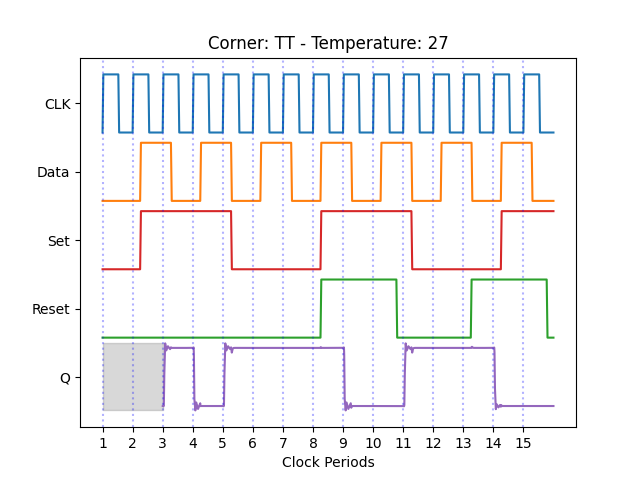
\includegraphics[width=\textwidth]{Figures/Aimspice_Plots/TT_27.png}
    \caption{Plot of register for TT corner}
    \label{fig:result_TT27}
\end{figure}

As shown in figure \ref{fig:result_TT27} and figure \ref{fig:result_FF27}, the different combinations of the inputs signals. If set is high, Q only updates to the D-value when the CLK changes from low to high. And if the reset is high, the value Q is overruled to low, even if set and D is high.

When looking at the different corners and temperatures, the difference of the functionality is quite similar. One can see in this case with the TT and FF corners at 27$^\circ C$, that the register is just a tiny fraction more stable with a FF corner rather than a TT corner.

\begin{figure}[H]
    \centering
    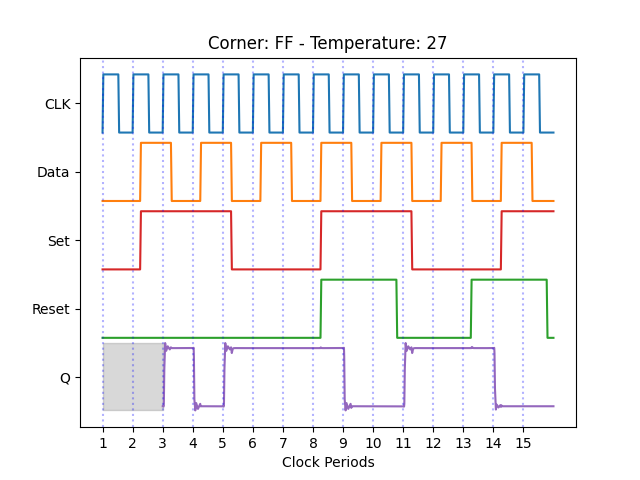
\includegraphics[width=\textwidth]{Figures/Aimspice_Plots/FF_27.png}
    \caption{Plot of register for FF corner}
    \label{fig:result_FF27}
\end{figure}

When simulation the static power consumption for the TT and FF corner, we look at a state where the CLK is not running and the inputs, D, S and R, are set to high. The static power consumption is calculated by taking the current in the VDD node and multiplying it with the VDD, as shown in equation \ref{eq:power}.

\begin{equation}
    \label{eq:power}
    P = I \cdot V
\end{equation}

For the TT corner, absolute value of the average current in the VDD node is $\approx$5 nA, and for the FF corner the absolute value of the average is $\approx$14 nA.

The static power consumption is therefore equal to $\approx$4.25 nW and $\approx$11.9 nW for the TT and FF corner respectively.

\begin{figure}[H]
\begin{minipage}{0.5\textwidth}
    \centering
    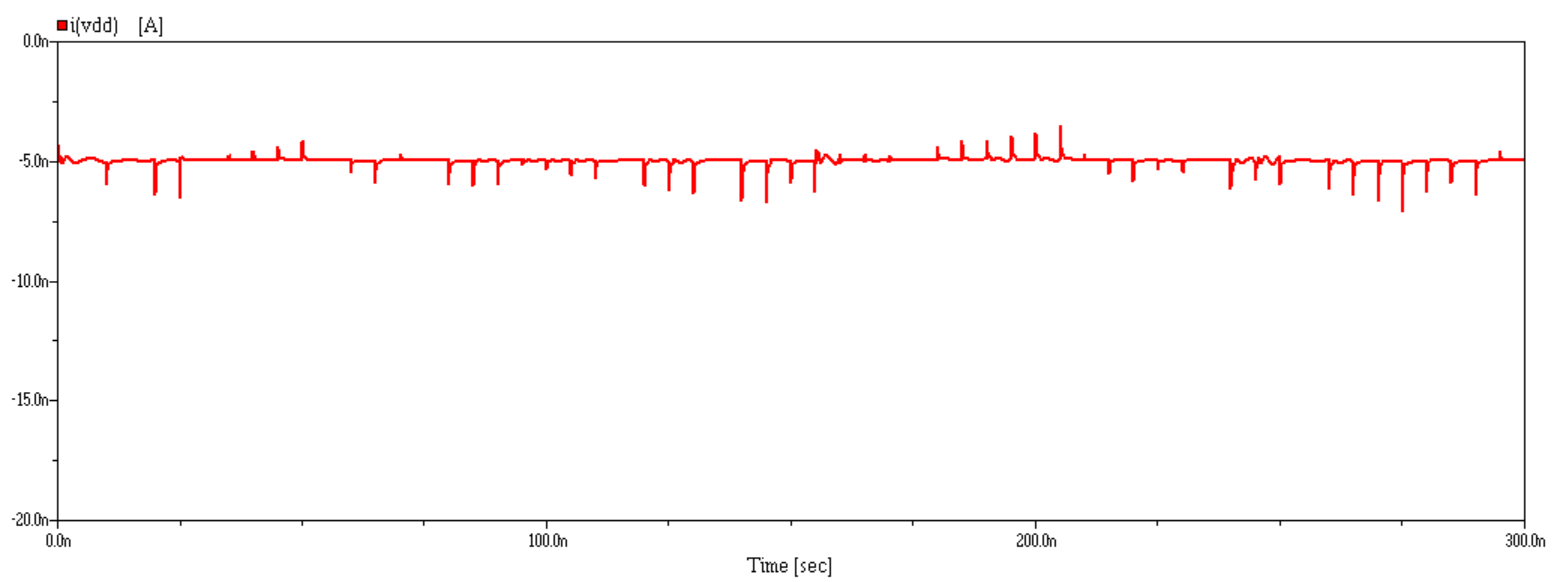
\includegraphics[width=\linewidth]{Figures/Current_VDD_TT.png}
    \caption{Current for TT corner}
    \label{fig:currentTT}
\end{minipage}
\begin{minipage}{0.5\textwidth}
    \centering
    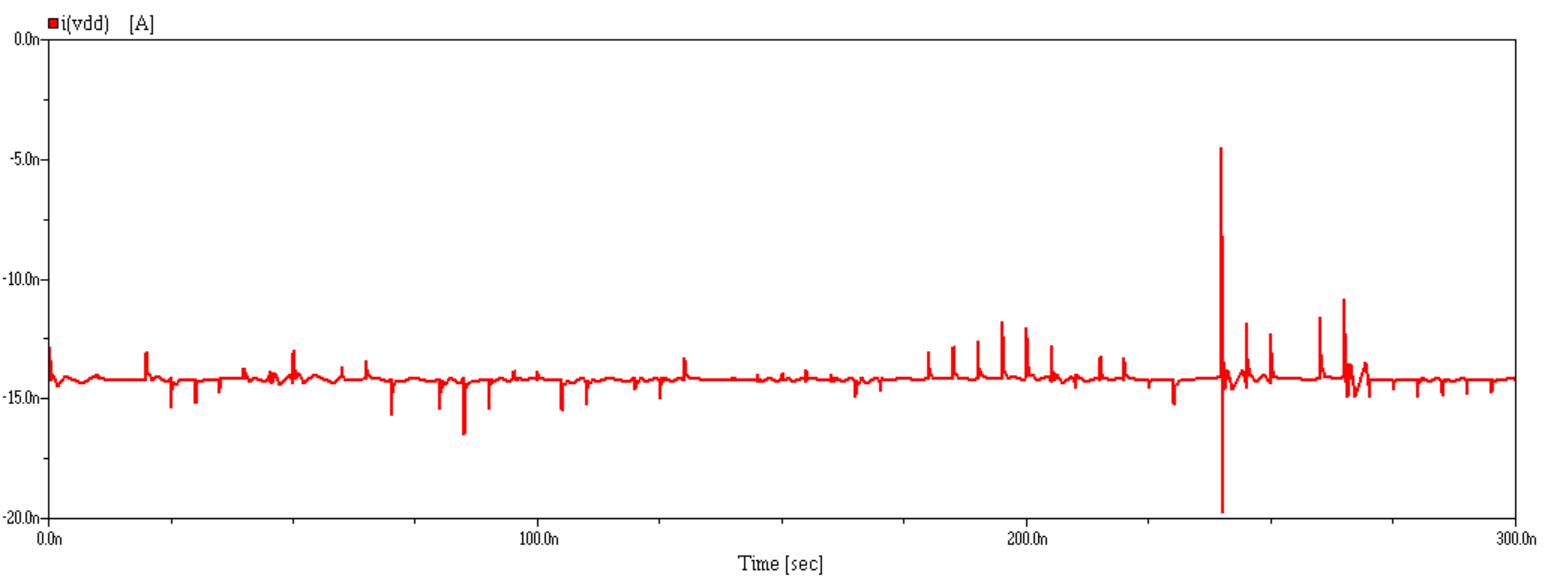
\includegraphics[width=\linewidth]{Figures/Current_VDD_FF.png}
    \caption{Current for FF corner}
    \label{fig:currentFF}
\end{minipage}
\end{figure}

\subsection{Verilog}

In this subsection results of Verilog-simulation will be presented. All Verilog-code is given in appendix~\ref{appendix:Verilog-code}.

Figure~\ref{fig:fsm_simulation} shows the FSM simulated for randomized inputs $I_1$ and $I_0$.

\begin{figure}[H]
    \centering
    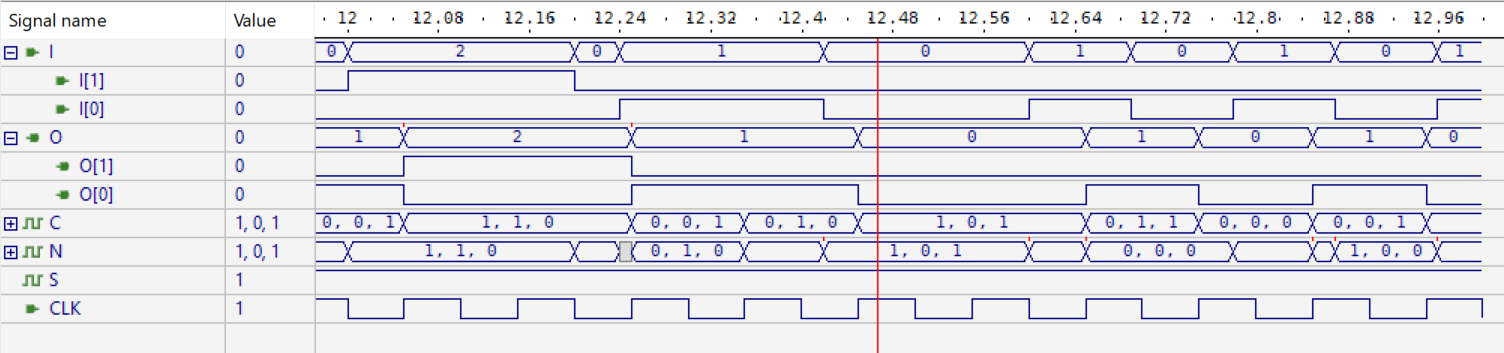
\includegraphics[width=\textwidth]{Figures/Test of FSM.png}
    \caption{Timing diagram of FSM simulated in Verilog}
    \label{fig:fsm_simulation}
\end{figure}

From the figure we see that the memory transitions to the expected states based on the inputs. The FSM begins in state ''Run-1'' and transitions to state ''Reset'' as the reset input $I_1$ is set high. The next state is ''Run-1'', then ''Run-2''. The Run-bit $I_0$ is then set low, resulting in a two-period pause in state ''Pause-2''. Further the FSM transitions to ''Run-3'', ''Pause'' and ''Run-1''.

This simulation was run and verified to follow the wanted behaviour as given by table~\ref{tab:truthtable}.

Figure~\ref{fig:eightbitadder_sim} shows a simulation of the 8-bit adder with random 8-bit inputs A and B. Note that all values in the timing diagram are hexadecimal and that any overflow-bits are handled outside our system. The code used for this simulation is given in listing~\ref{verilog_8bitadder}.

\begin{figure}[H]
    \centering
    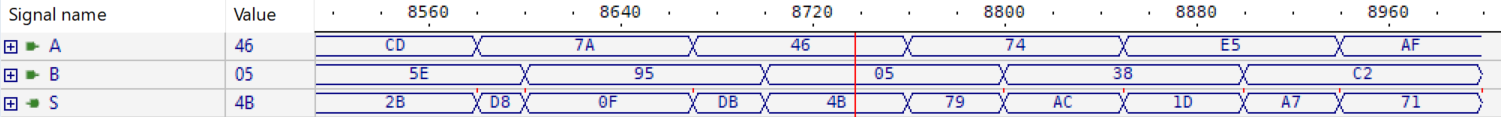
\includegraphics[width=\textwidth]{Figures/Test of eightbitadder.png}
    \caption{Timing diagram of 8-bit adder simulated in Verilog}
    \label{fig:eightbitadder_sim}
\end{figure}

Figure~\ref{fig:dflipflop_sim} shows a simulation of a single D Flip-Flop realized in Verilog.

\begin{figure}[H]
    \centering
    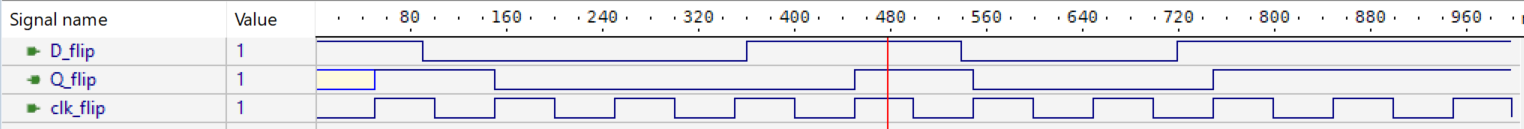
\includegraphics[width=\textwidth]{Figures/Test of Dflipflop.png}
    \caption{Timing diagram of D Flip-Flop simulated in Verilog}
    \label{fig:dflipflop_sim}
\end{figure}

Figure \ref{fig:8bitregister_sim} shows a simulation of a 8-bit register realized in Verilog.

\begin{figure}[H]
    \centering
    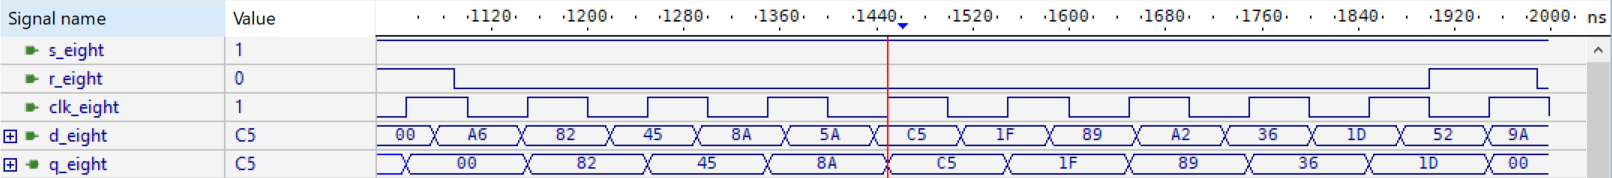
\includegraphics[width=\textwidth]{Figures/VerilogPlot_8bitreg.png}
    \caption{Timing diagram of an 8-bit register simulated in Verilog}
    \label{fig:8bitregister_sim}
\end{figure}

Figure~\ref{fig:multiplier_sim} shows a simulation of the 2-bit multiplier realized in Verilog. Inputs A and B are stimulated with arbitrary two bit values to observe the possible outputs. The multiplier has a 4-bit output as the largest possible output result, 9, needs four bits to be represented in binary.

\begin{figure}[H]
    \centering
    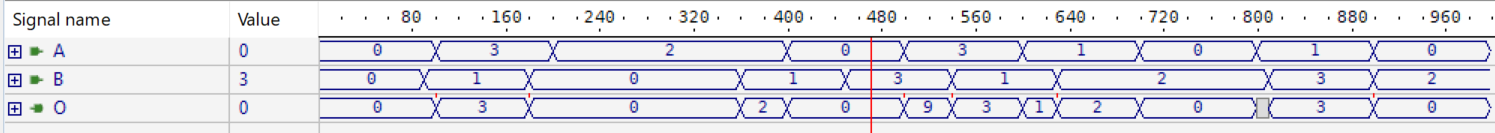
\includegraphics[width=\textwidth]{Figures/Test of multiplier.png}
    \caption{Timing diagram of multiplier simulated in Verilog}
    \label{fig:multiplier_sim}
\end{figure}



% Present the results of your simulations in this section. Use tables and graphs or other figures to illustrate your results. Remember: The table caption goes above the table, the figure caption goes below the figure.

% The results section must include:
% \begin{itemize}
%     \item Figures and/or tables that show the results of your simulation.
%     \item Text that describe what we see in the simulation results (e.g. as expected we can see that XYZ which means the circuit functions as intended).
%     \item NB! The result section is a \textit{what?}-section. \textit{What} where the results? \textit{What} do the figures/results mean? Any \textit{why}-questions you might want to write about and try to answer typically belong in the discussion section.
% \end{itemize}